\subsection{Snippet-level classification}
\label{sec:snippet-level}

The probability $\hat{Y}_k$ that a patient presents generalizing%
\footnote{Here `generalizing' refers to the seizure propagating to both hemispheres, not to the concept of machine learning models generalizing to data from different distributions.}
features within snippet $\x_k$ starting at frame $k$ is computed as
\begin{equation}
    \Ypred_k = \Pr(Y_k = 1 \mid \x_k) = \Fzx( \Cx(\x_k) ) = \Fzx( \z_k)
\end{equation}
where
$\Cx$ is an \ac{STCNN} parameterized by $\pars{\x}$ that extracts features from a snippet,
$\z_k \in \R ^ m$ is a vector of $m$ features representing $\x_k$ in a latent space,
and
$\Fzx$ is a fully-connected layer parameterized by $\pars{\z,\x}$ followed by a sigmoid function that maps logits to probabilities.
In this work, we do not update $\pars{\x}$ during training.


\subsection{Seizure-level classification}
\label{sec:meth_seizure}

\Cref{fig:gestures} shows an overview of our architecture for seizure-level classification.

\begin{figure}
  \centering
  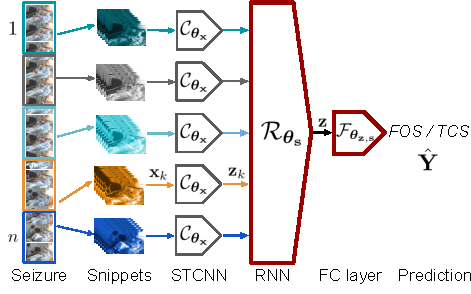
\includegraphics[width=0.8\textwidth]{diagram_gestures}
  \caption[Overview of the GESTURES architecture]{
    Overview of our architecture for seizure-level classification, which we name \acf*{GESTURES}.
    We train only the models with thick red borders.
    The video is split into $n$ segments of equal duration.
    A snippet $\x_k$ is sampled from each segment.
    Each snippet is fed to the feature extractor $\Cx$, which outputs a feature vector $\z_k$.
    The sequence of feature vectors is aggregated using a \acf*{RNN} $\Rs$ to produce a single feature vector $\z$, which is passed to a fully-connected (FC) layer $\Fzs$ to produce a prediction $\hat{\Yb}$ representing a \acf*{FOS} or a \acf*{FBTCS}.
  }
  \label{fig:gestures}
\end{figure}

\subsubsection{Temporal segment network}
Let $V = \{ \x_k \}_{k=1}^{K-l}$ be the set of all possible snippets sampled from a seizure video.
We define a sampling function $f : (V, n, \gamma) \mapsto S$ that extracts a sequence $S$ of $n$ snippets by splitting $V$ into $n$ non-overlapping segments and randomly sampling one snippet per segment.
There are two design choices: the number of segments $n$ and the probability distribution used for sampling within a segment.
If a uniform distribution is used, the last snippet from a segment and the first from the next could potentially be sampled, and very little variation would be expected between them, making information from two adjacent segments redundant.
Using always the middle snippet of a segment minimizes redundancy, but reduces the proportion of data leveraged during training.
We propose using a symmetric beta distribution ($\text{Beta}(\gamma, \gamma)$) to model the sampling function, where $\gamma$ controls the dispersion of the probability distribution (\cref{fig:betas}).
The set of latent snippet representations is $Z = \{ \Cx (\x_i) \}_{i = 1}^{n}$.


\subsubsection{Recurrent neural network}

To perform a seizure-level prediction $\hat{\Yb}$, $Z$ is aggregated as follows:
\begin{equation}
    \hat{\Yb}
    = \Pr(\Yb = 1 \mid S)
    = \Fzs( \Rs ( Z ) )
    = \Fzs( \z )
\end{equation}
where
$\Rs$ is an \ac{RNN} parameterized by $\pars{\sss}$,
$\Fzs$ is a fully-connected layer parameterized by $\pars{\z,\sss}$ which uses a softmax function to output probabilities,
and $\z$ is a feature-vector representation of the entire seizure video, corresponding to the last hidden state of $\Rs$.
